\documentclass{beamer}
\usepackage{tikz,amsmath,hyperref,graphicx,stackrel}
\usetikzlibrary{positioning,shadows,arrows,shapes,calc}
\newcommand{\argmax}{\operatornamewithlimits{argmax}}
\newcommand{\argmin}{\operatornamewithlimits{argmin}}
\mode<presentation>{\usetheme{Frankfurt}}
\AtBeginSection[]
{
  \begin{frame}<beamer>
    \frametitle{Outline}
    \tableofcontents[currentsection,currentsubsection]
  \end{frame}
}
\title{Lecture 4: Review of Linear Algebra}
\author{Mark Hasegawa-Johnson}
\date{ECE 417: Multimedia Signal Processing, Fall 2021}  
\begin{document}

% Title
\begin{frame}
  \maketitle
\end{frame}

\begin{frame}
Reading: \href{http://math.mit.edu/~gs/linearalgebra/linearalgebra5_6-1.pdf}{\bf\color{blue}Strang, Section 6.1}}
\end{frame}

% Title
\begin{frame}
  \tableofcontents
\end{frame}


%%%%%%%%%%%%%%%%%%%%%%%%%%%%%%%%%%%%%%%%%%%%
\section[Linear Algebra]{Review: Linear Algebra}
\setcounter{subsection}{1}
\begin{frame}
  \begin{columns}[t]
    \column{2.75in}
    \begin{block}{}
      A linear transform $\vec{y}=A\vec{x}$ maps vector space $\vec{x}$
      onto vector space $\vec{y}$.  For example: the matrix
      $A=\left[\begin{array}{cc}1 & 1\\0&2\end{array}\right]$
      maps the vectors $\vec{x}_0,\vec{x}_1,\vec{x}_2,\vec{x}_3=$
      \[
      \left[\begin{array}{c}1\\0\end{array}\right],
      \left[\begin{array}{c}\frac{1}{\sqrt{2}}\\\frac{1}{\sqrt{2}}\end{array}\right],
      \left[\begin{array}{c}0\\1\end{array}\right],
      \left[\begin{array}{c}-\frac{1}{\sqrt{2}}\\\frac{1}{\sqrt{2}}\end{array}\right]
      \]
      to the vectors
      $\vec{y}_0,\vec{y}_1,\vec{y}_2,\vec{y}_3=$
      \[
      \left[\begin{array}{c}1\\0\end{array}\right],
      \left[\begin{array}{c}\sqrt{2}\\\sqrt{2}\end{array}\right],
      \left[\begin{array}{c}1\\2\end{array}\right],
      \left[\begin{array}{c}0\\\sqrt{2}\end{array}\right]
      \]
    \end{block}
    \column{1.5in}
    \begin{block}{}
      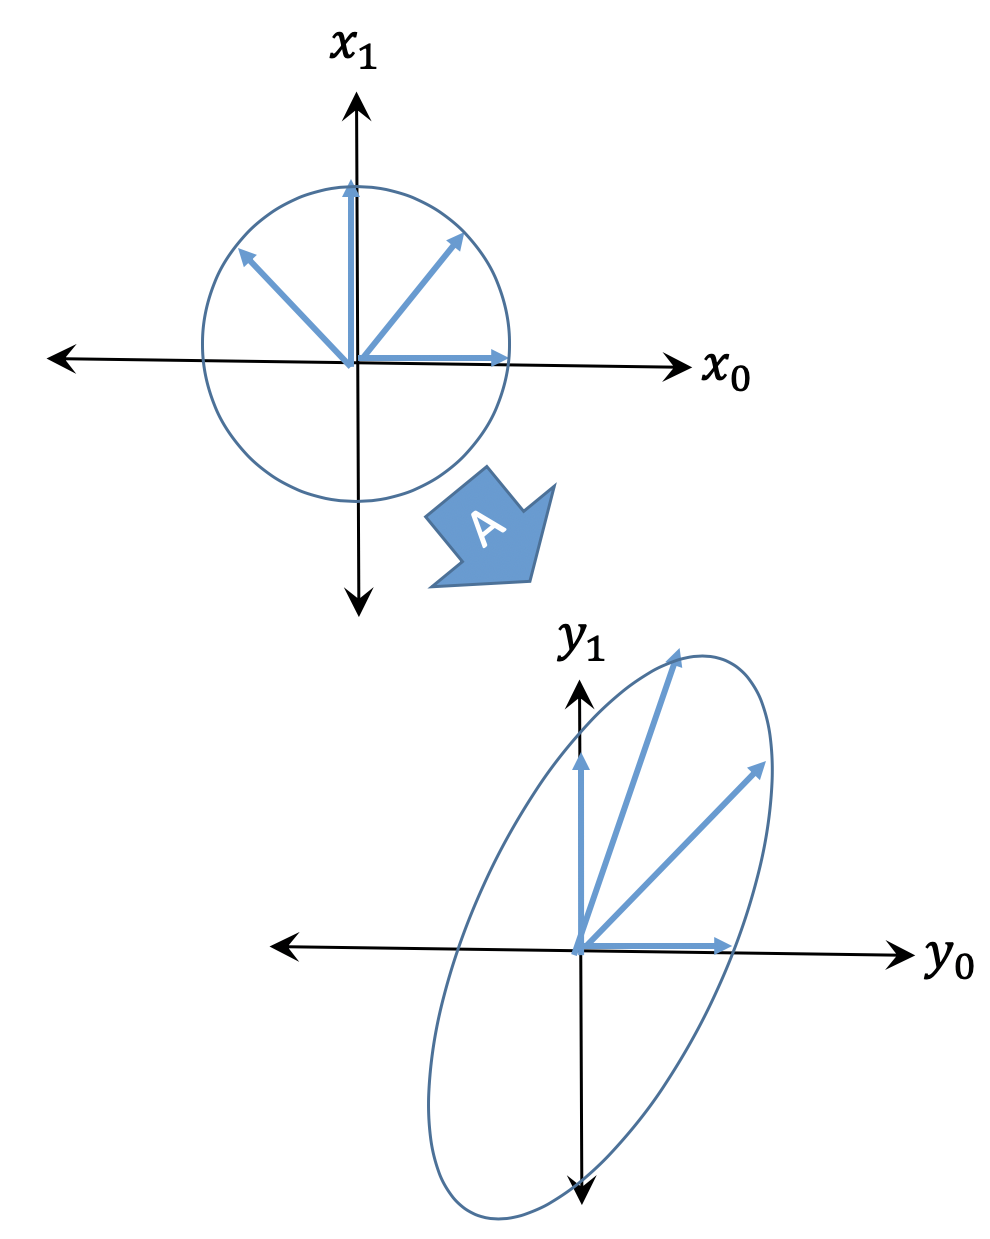
\includegraphics[width=1.45in]{linalg_review_fig1.png}
    \end{block}
  \end{columns}
\end{frame}

\begin{frame}
  \begin{columns}[t]
    \column{2.75in}
    \begin{block}{}
      A linear transform $\vec{y}=A\vec{x}$ maps vector
      space $\vec{x}$ onto vector space $\vec{y}$.  The absolute value of the
      determinant of $A$ tells you how much the area of a unit circle is
      changed under the transformation.
      
      For example, if
      $A=\left[\begin{array}{cc}1&1\\0&2\end{array}\right]$, then the
      unit circle in $\vec{x}$ (which has an area of $\pi$) is mapped to
      an ellipse with an area that is $\mbox{abs}(|A|)=2$ times larger, i.e.,
      i.e., $\pi\mbox{abs}(|A|)=2\pi$.
    \end{block}
    \column{1.5in}
    \begin{block}{}
      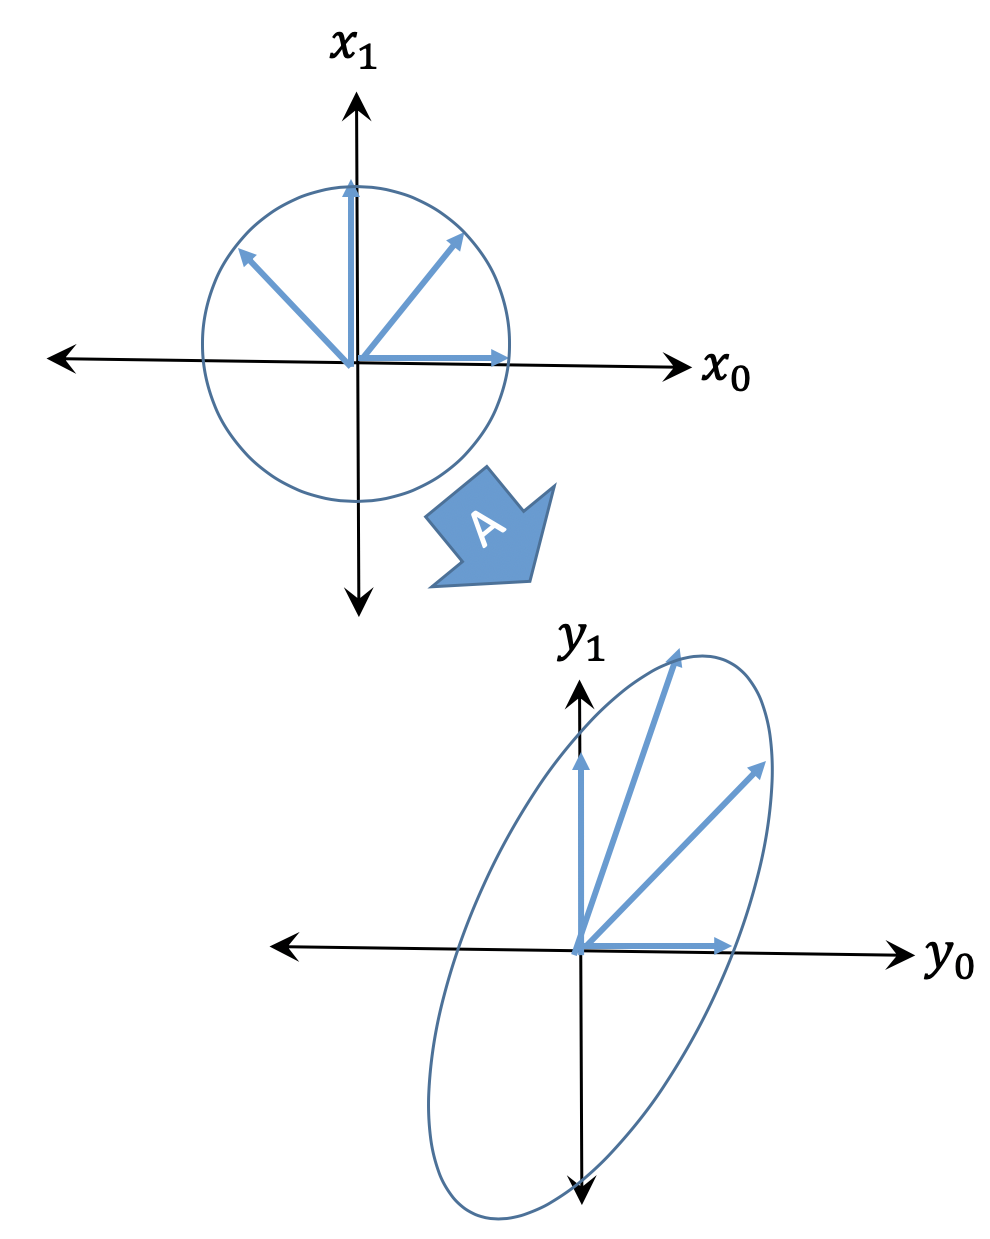
\includegraphics[width=1.45in]{linalg_review_fig1.png}
    \end{block}
  \end{columns}
\end{frame}

\begin{frame}
  \begin{columns}[t]
    \column{2.75in}
    \begin{block}{}
      For a D-dimensional square matrix, there may be up to $D$
        different directions $\vec{x}=\vec{v}_d$ such that, for some
        scalar $\lambda_d$, $A\vec{v}_d=\lambda_d\vec{v}_d$.
        For example, if
        $A=\left[\begin{array}{cc}1&1\\0&2\end{array}\right]$, then the
        eigenvectors are
        \[
        \vec{v}_0=\left[\begin{array}{c}1\\0\end{array}\right],~~
        \vec{v}_1=\left[\begin{array}{c}\frac{1}{\sqrt{2}}\\\frac{1}{\sqrt{2}}\end{array}\right],~~
        \]
        and the eigenvalues are $\lambda_0=1$, $\lambda_1=2$.
        Those vectors are red and extra-thick, in the figure to the
        left.  Notice that one of the vectors gets scaled by $\lambda_0=1$, but
        the other gets scaled by $\lambda_1=2$.
    \end{block}
    \column{1.5in}
    \begin{block}{}
      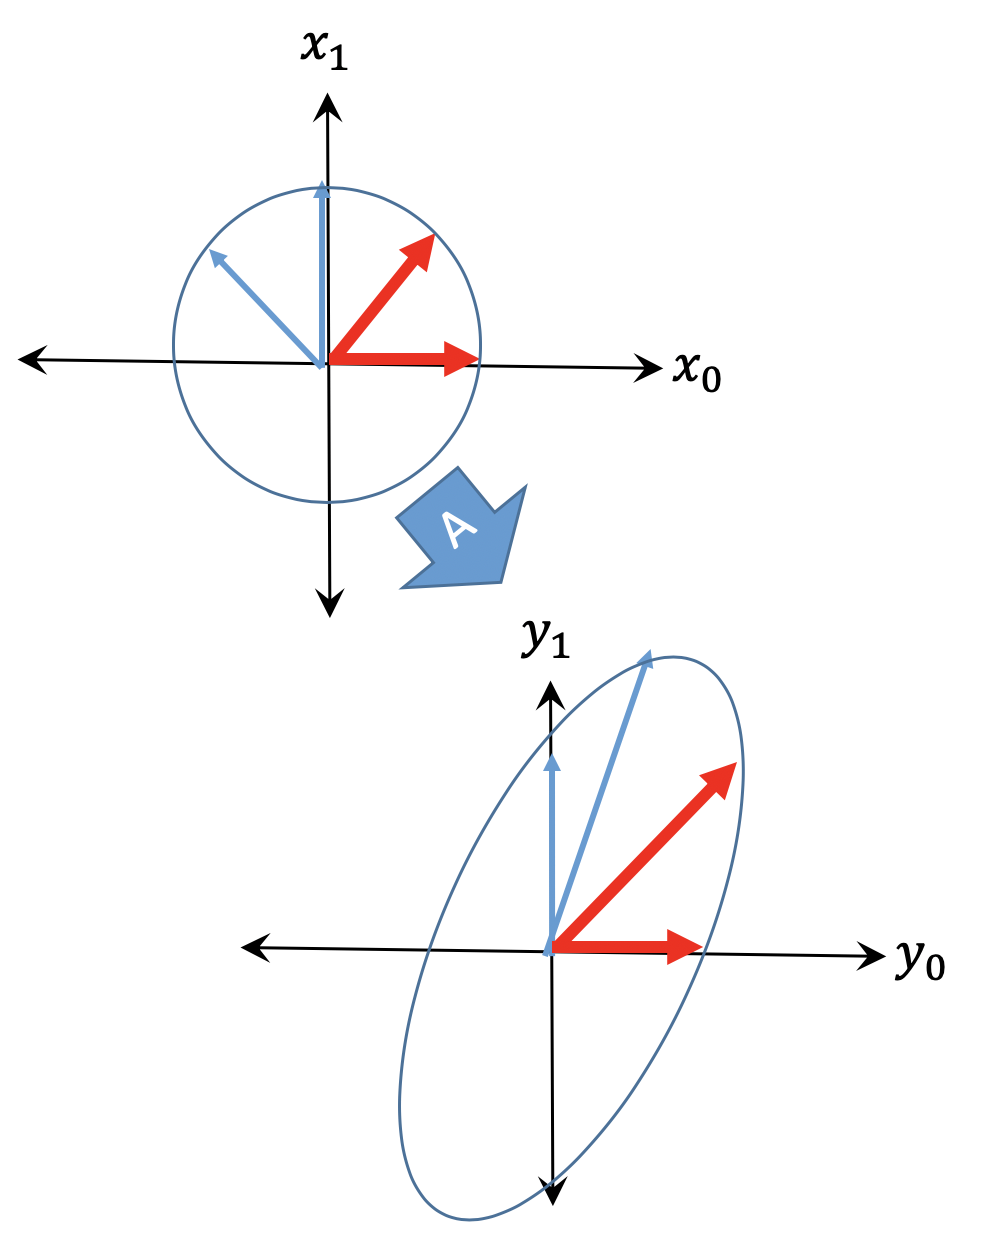
\includegraphics[width=1.45in]{linalg_review_fig2.png}
    \end{block}
  \end{columns}
\end{frame}

\begin{frame}
  \begin{columns}[t]
    \column{2.75in}
    \begin{block}{}
        An eigenvector is a direction, not just a vector.  That means
        that if you multiply an eigenvector by any scalar, you get the
        same eigenvector: if $A\vec{v}_d=\lambda_d\vec{v}_d$, then it’s
        also true that $cA\vec{v}_d=c\lambda_d\vec{v}_d$ for any scalar $c$.
        For example: the following are the same eigenvector as $\vec{v}_1$
        \[
        \sqrt{2}\vec{v}_1=\left[\begin{array}{c}1\\1\end{array}\right],~~
        -\vec{v}_1=\left[\begin{array}{c}-\frac{1}{\sqrt{2}}\\-\frac{1}{\sqrt{2}}\end{array}\right]
        \]
        Since scale and sign don't matter, by convention, we normalize so that 
        an eigenvector is always unit-length ($\Vert\vec{v}_d\Vert=1$) and
        the first nonzero element is non-negative ($v_{d0}>0$).
    \end{block}
    \column{1.5in}
    \begin{block}{}
      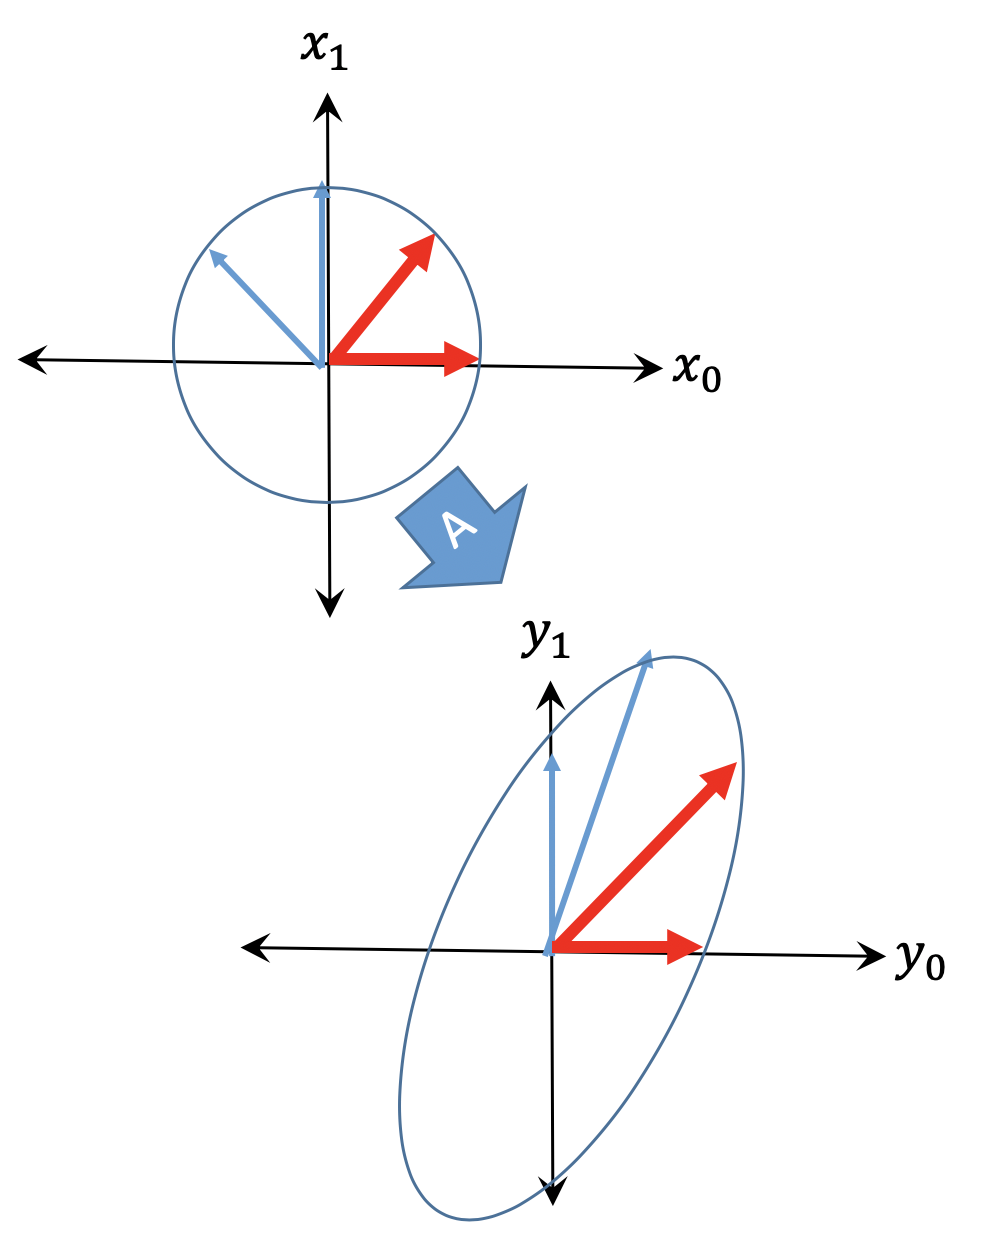
\includegraphics[width=1.45in]{linalg_review_fig2.png}
    \end{block}
  \end{columns}
\end{frame}

\begin{frame}
  \begin{columns}[t]
    \column{2.75in}
    \begin{block}{}
      \noindent{\bf Eigenvalues:}
      Before you find the eigenvectors, you should first find
      the eigenvalues.  You can do that using this fact:
      \begin{align*}
        A\vec{v}_d &= \lambda_d\vec{v}_d\\
        A\vec{v}_d &= \lambda_d I\vec{v}_d\\
        A\vec{v}_d-\lambda_d I\vec{v}_d &=\vec{0}\\
        (A-\lambda_d I)\vec{v}_d &= \vec{0}
      \end{align*}
      That means that when you use the linear transform
      $(A-\lambda_d I)$ to transform the unit circle, the result has an
      area of $|A-\lambda I|=0$.
    \end{block}
    \column{1.5in}
    \begin{block}{}
      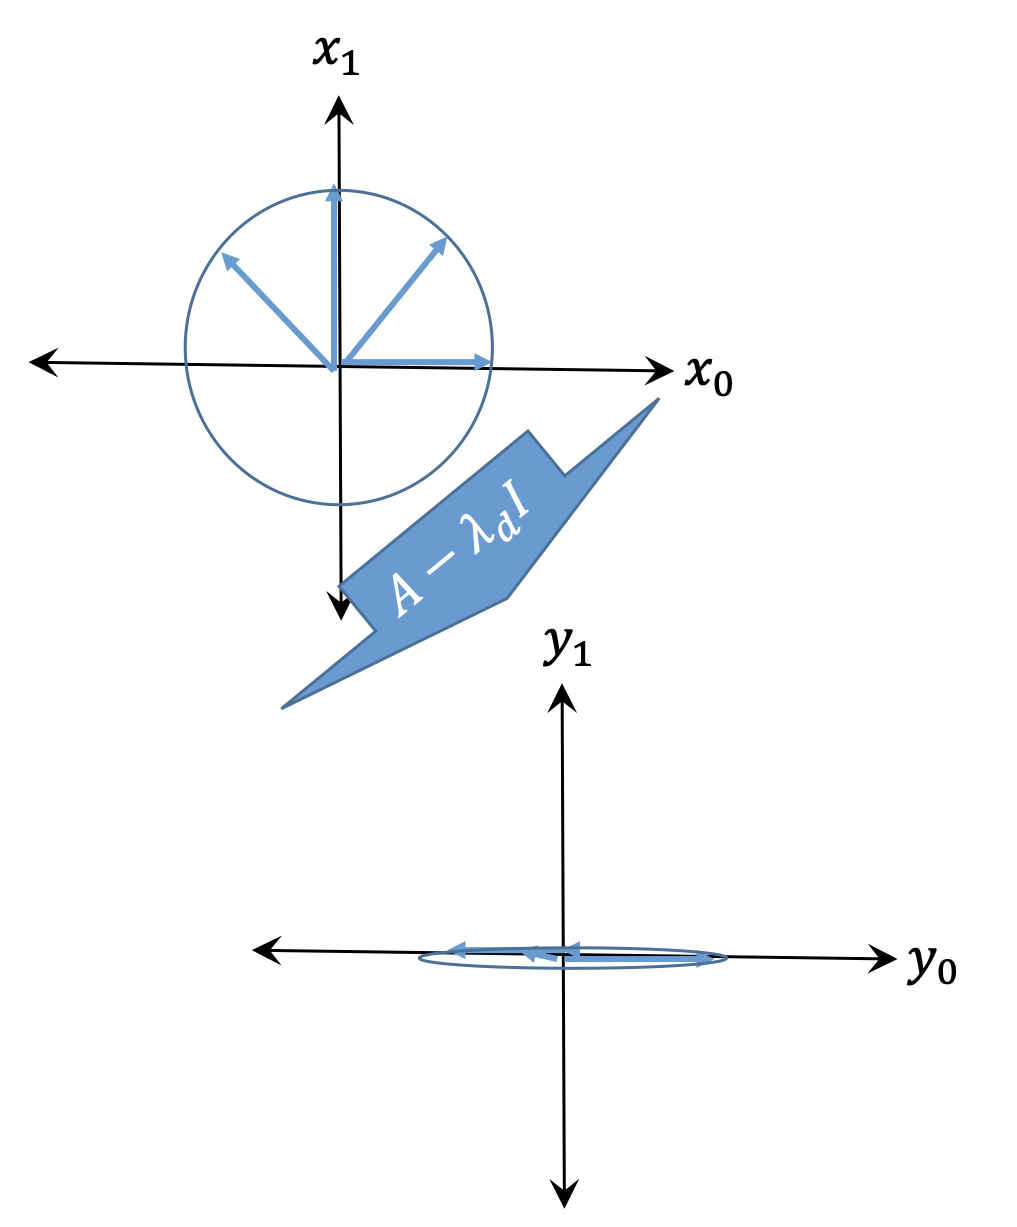
\includegraphics[width=1.45in]{linalg_review_fig3.png}
    \end{block}
  \end{columns}
\end{frame}

\begin{frame}
  \begin{columns}[t]
    \column{2.75in}
    \begin{block}{}
      \noindent{\bf Example:}
      \begin{align*}
        |A-\lambda I| &=
        \left|\begin{array}{cc}1-\lambda&1\\0&2-\lambda\end{array}\right|\\
        &=2-3\lambda+\lambda^2
      \end{align*}
      which has roots at $\lambda_0=1$, $\lambda_1=2$
    \end{block}
    \column{1.5in}
    \begin{block}{}
      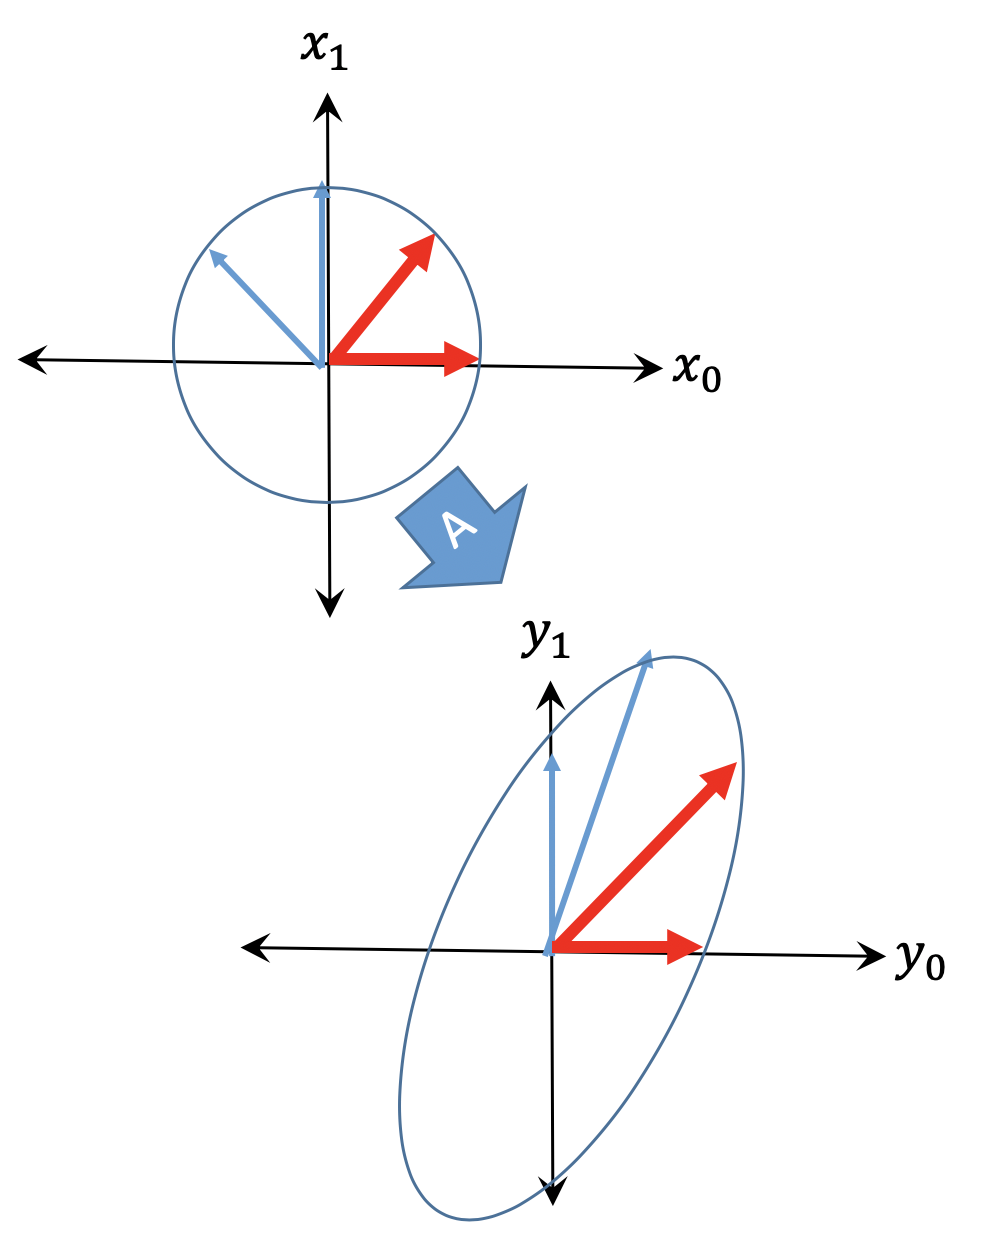
\includegraphics[width=1.45in]{linalg_review_fig2.png}
    \end{block}
  \end{columns}
\end{frame}

\begin{frame}
  \frametitle{There are always $D$ eigenvalues}
  \begin{itemize}
  \item The determinant $|A-\lambda I|$ is a $D^{\textrm{th}}$-order polynomial in $\lambda$.
  \item By the fundamental theorem of algebra, the equation
    \[
    |A-\lambda I|=0
    \]
    has exactly $D$ roots (counting repeated roots and complex roots).
  \item Therefore, {\bf any square matrix has exactly $D$ eigenvalues}
    (counting repeated eigenvalues, and complex eigenvalues.
  \end{itemize}
\end{frame}

\begin{frame}
  \frametitle{There are not always $D$ eigenvectors}

  Not every square matrix has $D$ eigenvectors.  Some of the most
  common exceptions are:
  \begin{itemize}
  \item {\bf Repeated eigenvalues:} if two of the roots of the
    polynomial are the same ($\lambda_j=\lambda_i$), then that means
    there is a two-dimensional subspace, $\vec{v}$, such that
    $A\vec{v}=\lambda_i\vec{v}$.  You can arbitrarily choose any two
    orthogonal vectors from this subspace to be the eigenvectors.
  \item {\bf Complex eigenvalues} correspond to complex eigenvalues.
    For example, the matrix
    \[
    A=\left[\begin{array}{cc}0&1\\-1&0\end{array}\right]
    \]
    has the eigenvalues $\lambda=\pm j$, and the corresponding eigenvectors
    \[
    \vec{v}_1=\frac{1}{\sqrt{2}}\left[\begin{array}{c}1\\j\end{array}\right],~~~
    \vec{v}_2=\frac{1}{\sqrt{2}}\left[\begin{array}{c}1\\-j\end{array}\right]
    \]
    Complex eigenvalues \& vectors require a little bit of extra notation that
    we'll mostly avoid dealing with.
  \end{itemize}
\end{frame}


%%%%%%%%%%%%%%%%%%%%%%%%%%%%%%%%%%%%%%%%%%%%%%%%%%%%%%%%%%%%%%%%%%%%%%%%%%%%%%%%%%%%%
\section[Eigenvectors]{Left and Right Eigenvectors}
\setcounter{subsection}{1}

\begin{frame}
  \frametitle{Review: Eigenvalues and eigenvectors}
  The eigenvectors of a $D\times D$ square matrix, $A$, are the
  vectors $\vec{v}$ such that
  \begin{equation}
    A\vec{v}=\lambda\vec{v}
    \label{eq:eigenvectors}
  \end{equation}
  The scalar, $\lambda$, is called the eigenvalue.  It's only possible
  for Eq.~(\ref{eq:eigenvectors}) to have a solution if
  \begin{equation}
    |A-\lambda I|=0
    \label{eq:eigenvalues}
  \end{equation}
\end{frame}

\begin{frame}
  \frametitle{Left and right eigenvectors}
  We’ve been working with right eigenvectors and right eigenvalues: 
  \[
  A\vec{v}_d =\lambda_d\vec{v}_d
  \]
  There may also be left eigenvectors, which are row vectors $\vec{u}_d$
  and corresponding left eigenvalues $\kappa_d$:
  \[
  \vec{u}_d^T A = \kappa_d\vec{u}_d^T
  \]
\end{frame}

\begin{frame}
  \frametitle{Eigenvectors on both sides of the matrix}
  You can do an interesting thing if you multiply the matrix by its eigenvectors both before and after:
  \[
  \vec{u}_i^T(A\vec{v}_j)=\vec{u}_i^T(\lambda_j\vec{v}_j)=\lambda_j\vec{u}_i^T\vec{v}_j
  \]
  \ldots but\ldots
  \[
  (\vec{u}_i^TA)\vec{v}_j=(\kappa_i\vec{u}_i^T)\vec{v}_j=\kappa_i\vec{u}_i^T\vec{v}_j
  \]
  There are only two ways that both of these things can be true. Either
  \[
  \kappa_i=\lambda_j~~~\mbox{or}~~~\vec{u}_i^T\vec{v}_j=0
  \]
\end{frame}

\begin{frame}
  \frametitle{Left and right eigenvectors must be paired!!}
  There are only two ways that both of these things can be true. Either
  \[
  \kappa_i=\lambda_j~~~\mbox{or}~~~\vec{u}_i^T\vec{v}_j=0
  \]
  Remember that eigenvalues solve $|A-\lambda_d I|=0$.  In almost all
  cases, the solutions are all distinct ($A$ has distinct
  eigenvalues), i.e., $\lambda_i\ne\lambda_j$ for $i\ne j$.  That
  means there is {\bf at most one} $\lambda_i$ that can equal each
  $\kappa_i$:
  \[
  \begin{cases}
    i\ne j & \vec{u}_i^T\vec{v}_j = 0\\
    i=j & \kappa_i = \lambda_i
  \end{cases}
  \]
\end{frame}

%%%%%%%%%%%%%%%%%%%%%%%%%%%%%%%%%%%%%%%%%%%%
\section[Symmetric]{Eigenvectors of symmetric matrices}
\setcounter{subsection}{1}

%\begin{frame}
%  \frametitle{Properties of symmetric matrices}
%  If $A$ is symmetric with $D$ eigenvectors, and $D$ distinct eigenvalues, then
%  \[
%  VV^T=V^TV=I
%  \]
%  \[
%  V^TAV = \Lambda
%  \]
%  \[
%  A=V\Lambda V^T
%  \]
%\end{frame}

\begin{frame}
  \frametitle{Symmetric matrices: left=right}

  If $A$ is symmetric ($A=A^T$), then the left and right eigenvectors
  and eigenvalues are the same, because
  \[
  \lambda_i\vec{u}_i^T=\vec{u}_i^TA=(A^T\vec{u}_i)^T=(A\vec{u}_i)^T
  \]
  $\ldots$ and that last term is equal to $\lambda_i\vec{u}_i^T$ if and
  only if $\vec{u}_i=\vec{v}_i$.
\end{frame}

\begin{frame}
  \frametitle{Symmetric matrices: eigenvectors are orthonormal}
  Let's combine the following facts:
  \begin{itemize}
  \item $\vec{u}_i^T\vec{v}_j=0$ for $i\ne j$ --- any square matrix with distinct
    eigenvalues
  \item $\vec{u}_i=\vec{v}_i$ --- symmetric matrix
  \item $\vec{v}_i^T\vec{v}_i=1$ --- standard normalization of
    eigenvectors for any matrix (this is what $\Vert\vec{v}_i\Vert=1$ means).
  \end{itemize}
  Putting it all together, we get that
  \[
  \vec{v}_i^T\vec{v}_j=
  \begin{cases}
    1&i=j\\
    0&i\ne j
  \end{cases}
  \]
\end{frame}

\begin{frame}
  \frametitle{The eigenvector matrix}
  So if $A$ is symmetric with distinct eigenvalues, then
  its eigenvectors  are orthonormal:
  \[
  \vec{v}_i^T\vec{v}_j=
  \begin{cases}
    1&i=j\\
    0&i\ne j
  \end{cases}
  \]
  We can  write this as
  \[
  V^TV = I
  \]
  where
  \[
  V=\left[\vec{v}_0,\ldots,\vec{v}_{D-1}\right]
  \]
\end{frame}

\begin{frame}
  \frametitle{The eigenvector matrix is orthonormal}
  \[
  V^TV = I
  \]
  \ldots and it also turns out that
  \[
  VV^T = I
  \]
  Proof: 
  $VV^T=VIV^T=V(V^TV)V^T=(VV^T)^2$, but the only matrix that satisfies
  $VV^T=(VV^T)^2$ is $VV^T=I$.
\end{frame}

\begin{frame}
  \frametitle{Eigenvectors orthogonalize a symmetric matrix}
  So now, suppose $A$ is symmetric:
  \[
  \vec{v}_i^TA\vec{v}_j=
  \vec{v}_i^T(\lambda_j\vec{v}_j)=\lambda_j\vec{v}_i^T\vec{v}_j
  =\begin{cases}\lambda_j,&i=j\\0,&i\ne j\end{cases}
  \]
  In other words, if a symmetric matrix has $D$ eigenvectors with
  distinct eigenvalues, then its eigenvectors orthogonalize $A$:
  \[
  V^TAV = \Lambda
  \]
  \[
  \Lambda=
  \left[\begin{array}{ccc}\lambda_0&0&0\\0&\ldots&0\\0&0&\lambda_{D-1}\end{array}\right]
  \]
\end{frame}

\begin{frame}
  \frametitle{A symmetric matrix is the weighted sum of its eigenvectors:}
  One more thing.  Notice that
  \[
  A = VV^TAVV^T =V\Lambda V^T
  \]
  The last term is
  \[
  \left[\vec{v}_0,\ldots,\vec{v}_{D-1}\right]
  \left[\begin{array}{ccc}\lambda_0&0&0\\0&\ldots&0\\0&0&\lambda_{D-1}\end{array}\right]  
  \left[\begin{array}{c}\vec{v}_0^T\\\vdots\\\vec{v}_{D-1}^T\end{array}\right]=
  \sum_{d=0}^{D-1}\lambda_d \vec{v}_d\vec{v}_d^T
  \]
\end{frame}

\begin{frame}
  \frametitle{Summary: properties of symmetric matrices}
  If $A$ is symmetric with $D$ eigenvectors, and $D$ distinct eigenvalues, then
  \[
  A=V\Lambda V^T
  \]
  \[
  \Lambda = V^TAV
  \]
  \[
  VV^T=V^TV=I
  \]
\end{frame}

%%%%%%%%%%%%%%%%%%%%%%%%%%%%%%%%%%%%%%%%%%%%%%%%%%%%%%%%%%%%%%%%%%%%%%%%%%%%%%%%%%%%%
\section{Examples}
\setcounter{subsection}{1}

\begin{frame}
  \frametitle{In-Lecture Written Example Problem}
  
  Pick an arbitrary $2\times 2$ symmetric matrix.  Find its
  eigenvalues and eigenvectors.  Show that $\Lambda=V^TAV$ and
  $A=V\Lambda V^T$.
\end{frame}
  
\begin{frame}
  \frametitle{In-Lecture Jupyter Example Problem}
  
  Create a jupyter notebook.  Pick an arbitrary $2\times 2$ matrix.
  Plot a unit circle in the $\vec{x}$ space, and show what happens to
  those vectors after transformation to the $\vec{y}$ space.
  Calculate the determinant of the matrix, and its eigenvalues and
  eigenvectors.  Show that $A\vec{v}=\lambda\vec{v}$.
  
\end{frame}
  
%%%%%%%%%%%%%%%%%%%%%%%%%%%%%%%%%%%%%%%%%%%%%%%%%%%%%%%%%%%%%%%%%%%%%%%%%%%%%%%%%%%%%
\section{Summary}
\setcounter{subsection}{1}

\begin{frame}
  \frametitle{Summary}
  \begin{itemize}
  \item A linear transform, $A$, maps vectors in space $\vec{x}$ to vectors in space $\vec{y}$.
  \item The determinant, $|A|$, tells you how the volume of the unit
    sphere is scaled by the linear transform.
  \item Every $D\times D$ linear transform has $D$ eigenvalues, which
    are the roots of the equation $|A-\lambda I|=0$.
  \item Left and right eigenvectors of a matrix are either orthogonal
    ($\vec{u}_i^T\vec{v}_j=0$) or share the same eigenvalue ($\kappa_i=\lambda_j$).
  \item For a symmetric matrix, the left and right eigenvectors are
    the same.  If the eigenvalues are distinct and real, then:
    \[
    A=V\Lambda V^T,~~~\Lambda = V^TAV,~~~VV^T=V^TV=I
    \]
  \end{itemize}
\end{frame}

\end{document}

